\documentclass{beamer}
\usepackage{predavanja}
% Naloga 1.3.1: Za dokument uporabite razred `beamer'.
% Ne dodajajte nastavitve za velikost pisave, kot je bila v datoteki `5-prosojnice.tex`.

% Naloga 1.3.2: vključite paket `predavanja'.

% Naloga 1.3.3: definirajte okolji `definicija' in `izrek'.
% Namig: z iskanjem po datotekah (Ctrl+Shift+F oz. Cmd+Shift+F) 
% poiščite niz `{definicija}' ali niz `{izrek}'.

\newtheorem{definicija}{Definicija}
\newtheorem{izrek}{Izrek}

\usepackage{tikz}
\usetikzlibrary{math}

\usepackage{pgfplots}
\usepgfplotslibrary{external}

\usepackage{array}   %dodatne možnosti za tabele

\newcommand{\ZZ}{\mathbb{Z}}
\newcommand{\RR}{\mathbb{R}}
\newcommand{\CC}{\mathbb{C}}

\begin{document}

% Naloga 1.3.4: pripravite naslovno stran z vsebino:
\title{Matematični izrazi in uporaba paketa \texttt{beamer}}
\subtitle{\emph{Matematičnih} nalog ni treba reševati!}
\institute{Fakulteta za matematiko in fiziko}
\date{}

% Zgornje podatke nastavite z ukazi kot v dokumentih razreda `article`.
% Več o tem, kako se naredi naslovno stran, si preberite na naslovu na naslovu:
% https://www.overleaf.com/learn/latex/Beamer
% To stran preberite do vključno razdelka "Creating a table of contents".
% Ukaz `\titlepage` deluje podobno kot ukaz `\maketitle`, ki ste ga že srečali.

\frame{\titlepage}

% Naloga 1.3.5: pripravite kazalo vsebine.
% 1. Naslov prosojnice, s kazalom vsebine naj bo "Kratek pregled"
% 2. S pomožnim parametrom `pausesections' (v oglatih oklepajih) 
%    določite, da naj se kazalo vsebine odkriva postopoma.
%    Poglejte, kako deluje ta ukaz.
% 3. Ker ni videti preveč lepo, pomožni parameter zakomentirajte.

\begin{frame}
   \frametitle{Kratek pregled}
   \tableofcontents %[pausesections]
\end{frame}


\section{Paket \texttt{beamer}}
%  Naslov prosojnice lahko naredimo tudi z dodatnim parametrom okolja `frame`.
\begin{frame}{Posebnosti prosojnic}
	% Naloga 2.3.1:
	% Dodajte ukaze, ki bodo poskrbeli, da se bo prosojnica odkrivala postopoma,
	% tako kot v datoteki prosojnice-resitev.pdf

	Za prosojnice je značilna uporaba okolja \texttt{frame},
	s katerim definiramo posamezno prosojnico,  \pause
	%
	postopno odkrivanje prosojnic, \pause
	%
	ter nekateri drugi ukazi, ki jih najdemo v paketu \texttt{beamer}. \pause
	%
	\begin{exampleblock}{Primer}   
		Verjetno ste že opazili, da za naslovno prosojnico niste uporabili
		ukaza \texttt{maketitle}, ampak ukaz \texttt{titlepage}.
	\end{exampleblock}
\end{frame}

\begin{frame}{Poudarjeni bloki}
	% Naloga 2.3.2:
	% Oblikujte poudarjena bloka z opombo in opozorilom.
    \begin{exampleblock}{Opomba}
		Okolja za poudarjene bloke so \texttt{block}, \texttt{exampleblock} in \texttt{alertblock}.
	\end{exampleblock}

	\begin{exampleblock}{Pozor!}
		Začetek poudarjenega bloka (ukaz \texttt{begin}) vedno sprejme 
		dva parametra: okolje in naslov bloka.
		Drugi parameter (za naslov) je lahko prazen. 
	\end{exampleblock}

\end{frame}

\begin{frame}{Tudi v predstavitvah lahko pišemo izreke in dokaze}
	% Naloga 2.3.2:
	% Oblikujte okolje itemize, tako da se bo njegova vsebina postopoma odkrivala.
	% Ne smete uporabiti ukaza `pause'.
	% Beseda `največje' naj bo poudarjena šele na četrti podprosojnici.

	\begin{izrek}
	   Praštevil je neskončno mnogo.
	\end{izrek}
	\begin{proof}   %okolje za dokaz
	   Denimo, da je praštevil končno mnogo.
	   	% S pomožnim parametrom <+-> lahko določimo, da se bodo 
		% elementi naštevanja odkrivali postopoma.
	   \begin{itemize}[<+->]   % [<+->] pokaže posamezne točke
		  \item Naj bo $p$ \alert<4>{največje} praštevilo.  %alert ima vpliv samo na 4. podprosojnici lahko npr <1-3>
		  \item Naj bo $q$ produkt števil $1$, $2$, \ldots, $p$.
		  \item Število $q+1$ ni deljivo z nobenim praštevilom, torej je $q+1$ praštevilo.
		  \item To je protislovje, saj je $q+1>p$. \qedhere    %kam naj se postavi znak za konec dokaza
	   \end{itemize}
	\end{proof}

\end{frame}
 

\section{Paketa \texttt{amsmath} in \texttt{amsfonts}}
\begin{frame}{Matrike}
	% Naloga 3.2.1:
	% Oblikujte determinanto matrike. 
	% Vsebina matrike je že pripravljena v komentarju spodaj.
	Izračunajte determinanto
	$$    %vklopi matematično okolje, za metematični izraz
    \begin{vmatrix}
		 -1 & 4 & 4 & -2 \\
		 1 & 4 & 5 & -1 \\
		 1 & 4 & -2 & 2 \\
		 3 & 8 & 4 & 3 
    \end{vmatrix}
	$$
	V pomoč naj vam bo Overleaf dokumentacija o matrikah:
	
	\href{https://www.overleaf.com/learn/latex/Matrices}{\beamergotobutton{Matrices}}
\end{frame}

\begin{frame}{Okolje \texttt{align} in \texttt{align*}}
	% Naloga 3.2.2:
	% Okolje align je namenjeno poravnavi enačb.
	% Če ne želimo, da se enačba oštevilči, uporabimo okolje align*.
	% Nadomestite prikazni matematični način z okoljem align*.
	% Na ustreznih mestih vključite & in \\, da bo enačba videti kot v rešitvi.
	% Za pravilno postopno odkrivanje morate na enem mestu uporabiti ukaz `only' samo za eno prosojnic,
	% ter na dveh mestih ukaz `onslide' določimo interval.

	Dokaži \emph{binomsko formulo}: za vsaki realni števili $a$ in $b$ in za vsako naravno število $n$ velja 
    \begin{align*}     %znotraj matematičnih okolij ne sme biti praznih vrstic
	(a+b)^n \only<1>{&= \ldots \\ }     %poravnava pri znakih &
	\onslide<2->{&= (a+b) (a+b) \dots (a+b) \\}    % \\ prelom strani
	\onslide<3->{&= a^n + n a^{n-1} b + \dots + \binom{n}{k} a^{n-k} b^k + \dots + n a b^{n-1} + b^n \\}
	&= \sum_{k=0}^n \binom{n}{k} a^{n-k} b^k
    \end{align*}
\end{frame}

\begin{frame}{Še ena uporaba okolja \texttt{align*}}
	% Naloga 3.2.3:
	% Oblikujte spodnje enačbe z okoljem align* , z * je brez številčenja.
	% Če naredite po en kurzor na začetku vsake vrstice, 
	% boste lahko oblikovali vse tri vrstice hkrati.
	Nariši grafe funkcij:
	\begin{align*}
	y &= x^2 - 3|x| + 2  &   y &= 3 \sin(\pi+x) - 2  \\
	y &= \log_2(x-2) + 3 &   y &= 2 \sqrt{x^2+15} + 6 \\
	y &= 2^{x-3} + 1     &   y &= \cos(x-3) + \sin^2(x+1) 
	\end{align*}
\end{frame}

\begin{frame}{Okolje \texttt{multline}}  %multline- formula čez več vrstic
	% Naloga 3.2.4:
	% Oblikujte spodnje enačbe z ustreznim okoljem,
	% da bo enačba oblikovana kot v rešitvah.
	Poišči vse rešitve enačbe
	\begin{multline*}
	(1+x+x^2) \cdot (1+x+x^2+x^3+\ldots+x^9+x^{10}) = \\
	=(1+x+x^2+x^3+x^4+x^5+x^6)^2.
	\end{multline*}
\end{frame}

\begin{frame}{Okolje \texttt{cases}}
	% Naloga 3.2.5:
	% Oblikujte spodnji funkcijski predpis z ustreznim okoljem,
	% da oblikovan kot v rešitvah.
	Dana je funkcija
	$$
	   f (x,y) =\begin{cases}  %naredi zaviti oklepaj
		    \frac{3x^2y-y^3}{x^2+y^2}; &(x, y) \ne (0, 0),\\
			a; & (x, y) = (0, 0).
		 \end{cases}
	$$
	\begin{itemize}
		% ukaz displaystyle preklopi v prikazni način v vrstici. 
	\item Določi $a$, tako da izračunaš limito \( \lim_{(x,y)\to(0,0)} f(x). \)
	\item Izračunaj parcialna odvoda $f_x(x,y)$ in $f_y(x,y)$.
	\end{itemize}
\end{frame}


\section[Matematika, 1. del\\\large{Analiza, logika, množice}]{Matematika, 1. del}
\begin{frame}{Logika in množice}
	\begin{enumerate}
		\item
		Poišči preneksno obliko formule 
		$\exists x :P(x) \land \forall x: Q(x) \Rightarrow \forall x: R(x) $.
		\item 
		Definiramo množici A = [2,5]  in  B = \{0, 1, 2, 3, 4, \dots\}.\\
		V ravnino nariši:
		\begin{enumerate}
		   \item $ A \cap B \times \emptyset$
		   \item $ (A \cup B)^c  \times \mathbb{R} $
		\end{enumerate}
		\item
		Dokaži:
		\begin{itemize}
			\item $ (A \Rightarrow B) \sim  (\lnot B \Rightarrow \lnot A )$
			\item $\lnot (A \lor B) \sim \lnot A \land \lnot B $
		\end{itemize}
	\end{enumerate}
\end{frame}

\begin{frame}{Analiza}
	\begin{enumerate}
		\item
		Pokaži, da je funkcija $ x \mapsto \sqrt{x}$  enakomerno zvezna na $ [0, \infty].$
		\item 
		Katero krivuljo določa sledeč parametričen zapis?
		% Spodaj si pomagajte z dokumentacijo o razmikih v matematičnem načinu.
		% https://www.overleaf.com/learn/latex/Spacing_in_math_mode
		$$
		   x(t) = a \cos t, \qquad % tu manjka ukaz za presledek ostali znaki \, \: \; \
		   y(t) = b \sin t, \qquad % tu manjka ukaz za presledek
		   t \in [0, 2 \pi]
		$$ 
		\item
		Pokaži, da ima $f(x) = 3x + \sin(2x)$ inverzno funkcijo in izračunaj $ (f^{-1})'(3\pi)$.
		% \sin da je napisan pokončno
		\item
		Izračunaj integral 
		% V rešitvah smo spodnji integral zapisali v vrstičnem načinu,
		% ampak v prikaznem slogu. To naredite tako, da v matematičnem načinu najprej
		% uporabite ukaz displaystyle.
		% Pred dx je presledek: pravi ukaz je \,
		$ \displaystyle {\int
		 {\frac{2+\sqrt{x+1}}{(x+1)^2-\sqrt{x+1}}}} \, dx$ 
		\item 
		Naj bo $g$ zvezna funkcija. Ali posplošeni integral 
		$ \int_{0}^{1}  {\frac{g(x)}{x^2}} $
		konvergira ali divergira? Utemelji.
	\end{enumerate}
\end{frame}

\begin{frame}{Kompleksna števila}
	\begin{enumerate}
		\item
		Naj bo $z$ kompleksno število, $z \ne 1$ in $|z| = 1$.
		Dokaži, da je število \( i \, \frac{z+1}{z-1} \) realno.
		\item
		Poenostavi izraz:
		$$ 
		   \frac{\dfrac{3+i}{2-2i}+\dfrac{7i}{1-i}}{1+\dfrac{i-1}{4}-\dfrac{5}{2-3i}} 
		$$

        
	\end{enumerate}
\end{frame}


\section{Stolpci in slike}
\begin{frame}{Konstrukcija pravokotnice na premico $p$ skozi točko $T$}
    \begin{columns}
		\begin{column}{0.55\textwidth}
		  \begin{itemize}  % [<+->]  odkriva se postopoma
			 \item <1->Dani sta premica $p$ in točka $T$.
			 \item <2->Nariši lok $k$ s središčem v $T$.
			 \item <3->Premico $p$ seče v točkah $A$ in $B$.
			 \item <4->Nariši lok $m$ s središčem v $A$.
			 \item <5->Nariši lok $n$ s središčem v $B$ in z enakim polmerom.
			 \item <6->Loka se sečeta v točki $C$.
			 \item <7->Premica skozi točki $T$ in $C$ je pravokotna na $p$.
		  \end{itemize}
		\end{column}
        \begin{column}{0.45\textwidth}
			\centering
		   \includegraphics<1>[width=50mm]{slike/fig-1.png}%
		   \includegraphics<2>[width=50mm]{slike/fig-2.png}%
		   \includegraphics<3>[width=50mm]{slike/fig-3.png}%
		   \includegraphics<4>[width=50mm]{slike/fig-4.png}%
		   \includegraphics<5>[width=50mm]{slike/fig-5.png}%
		   \includegraphics<6>[width=50mm]{slike/fig-6.png}%
		   \includegraphics<7>[width=50mm]{slike/fig-7.png}%      % procent ignorira prskok vrstice
		\end{column}
	\end{columns}
\end{frame}

\begin{frame}{Konstrukcija pravokotnice na premico $p$ skozi točko $T$}
    \begin{columns}
		\begin{column}{0.55\textwidth}
		  \begin{itemize}  % [<+->]  odkriva se postopoma
			 \item <1->Dani sta premica $p$ in točka $T$.
			 \item <2->Nariši lok $k$ s središčem v $T$.
			 \item <3->Premico $p$ seče v točkah $A$ in $B$.
			 \item <4->Nariši lok $m$ s središčem v $A$.
			 \item <5->Nariši lok $n$ s središčem v $B$ in z enakim polmerom.
			 \item <6->Loka se sečeta v točki $C$.
			 \item <7->Premica skozi točki $T$ in $C$ je pravokotna na $p$.
		  \end{itemize}
		\end{column}
        \begin{column}{0.45\textwidth}
			\centering
			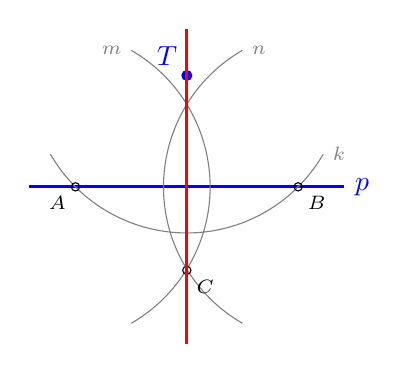
\begin{tikzpicture}
			     % Sliko smo naredili tako, da so točke A, B, T in C vse enako oddaljene
				 % od presečišča premic; kot ATC je 45°.
				 % Vsi krožni loki imajo radij 2.
				 \tikzmath{
				 	% Razdalja od točke T do premice p je tako 2*sin(45°).
				 	\t = 2*sin(45);
				 	% Razdalja začetka loka m do premice p
				 	% oz. razdalja točke T' levo in zgoraj od točke T do premice
				 	\tt = 2*sin(60);
				 	% Razdalja točke T' od navpične premice skozi T
				 	\td = \t-2*cos(60);
				 }
				 % Definicija točke T
				 \coordinate [label={[blue, above left]:$T$}] (T) at (0,{\t});  %da se izpiše T

				 % Risanje točke T
				 \fill[blue] (T) circle (2pt);

				 % Premica p
				 \draw[blue, very thick] (-2,0) -- (2,0) node[right] {$p$};  %{$p$} da se izpiše tudi oznaka
				 \pause

				 % Definicija pomožne točke A' in risanje krožnega loka k (arc), ki se začne v A'
				 \coordinate (A') at ({-\tt},{\td});
				 \draw[gray, thin] (A') arc[start angle=210, end angle=330, radius=2] node[right] {\scriptsize $k$};
				 \pause

				 % Točka A
				 \coordinate [label=below left:{\scriptsize $A$}] (A) at ({-\t},0);
				 \draw (A) circle (1.5pt);
				
				 % Naloga 3.4.1.: Narišite še točko B (skupaj z oznako)
				 \coordinate [label=below right:{\scriptsize $B$}] (B) at ({\t},0);
				 \draw (B) circle (1.5pt);
				 \pause

				 % Naloga 3.4.2.: Definirajte točko T', v kateri se začne lok m in narišite lok m z oznako.
				 % Lok je definiran s točko, v kateri se lok začne (ne središče!), z začetnim in končnim kotom ter radijem.
				 % Koti so vedno podani enako: kot 0 je v smeri x osi in se veča v nasprotni smeri urinega kazalca.
				 \coordinate (T') at ({-1.7*\td},{\tt});
				 \draw[gray, thin] (T') node[left] {\scriptsize $m$} arc[start angle=60, end angle=-60, radius=2] ;
				 \pause

				 % Naloga 3.4.3.: Definirajte točko T'' in narišite lok n z oznako.
				 \coordinate (T'') at ({1.7*\td},{\tt});
				 \draw[gray, thin] (T'') node[right] {\scriptsize $n$} arc[start angle=120, end angle=240, radius=2] ;
				 \pause

				 % Naloga 3.4.4.: Definirajte in narišite točko C.
				 \coordinate [label=below right:{\scriptsize $C$}] (C) at (0,{-0.75*\t});
				 \draw (C) circle (1.5pt);
				 \pause

				 % Naloga 3.4.5.: Narišite premico skozi točki T in C.
				 \draw[red, very thick] (0,-2) -- (0,2) ;

			\end{tikzpicture}
		\end{column}
	\end{columns}
\end{frame}

				% Spodnje je za nalogo 3.4.

				% % Sliko smo naredili tako, da so točke A, B, T in C vse enako oddaljene
				% % od presečišča premic; kot ATC je 45°.
				% % Vsi krožni loki imajo radij 2.
				% \tikzmath{
				% 	% Razdalja od točke T do premice p je tako 2*sin(45°).
				% 	\t = 2*sin(45);
				% 	% Razdalja začetka loka m do premice p
				% 	% oz. razdalja točke T' levo in zgoraj od točke T do premice
				% 	\tt = 2*sin(60);
				% 	% Razdalja točke T' od navpične premice skozi T
				% 	\td = \t-2*cos(60);
				% }
				% % Definicija točke T
				% \coordinate [label={[blue, above left]:$T$}] (T) at (0,{\t});
				% % Risanje točke T
				% \fill[blue] (T) circle (2pt);
				% % Premica p
				% \draw[blue, very thick] (-2,0) -- (2,0) node[right] {$p$};
				% \pause
				% % Definicija pomožne točke A' in risanje krožnega loka k, ki se začne v A'
				% \coordinate (A') at ({-\tt},{\td});
				% \draw[gray, thin] (A') arc[start angle=210, end angle=330, radius=2] node[right] {\scriptsize $k$};
				% \pause
				% % Točka A
				% \coordinate [label=below left:{\scriptsize $A$}] (A) at ({-\t},0);
				% \draw (A) circle (1.5pt);
				
				% % Naloga 3.4.1.: Narišite še točko B (skupaj z oznako)
				
				% % Naloga 3.4.2.: Definirajte točko T', v kateri se začne lok m in narišite lok m z oznako.
				% % Lok je definiran s točko, v kateri se lok začne (ne središče!), z začetnim in končnim kotom ter radijem.
				% % Koti so vedno podani enako: kot 0 je v smeri x osi in se veča v nasprotni smeri urinega kazalca.

				% % Naloga 3.4.3.: Definirajte točko T'' in narišite lok n z oznako.
				
				% % Naloga 3.4.4.: Definirajte in narišite točko C.

				% % Naloga 3.4.5.: Narišite premico skozi točki T in C.

				% Konec vsebine za nalogo 3.4.


% Naloga 4
 \begin{frame}{Graf funkcije s TikZ}
 	\centering
 	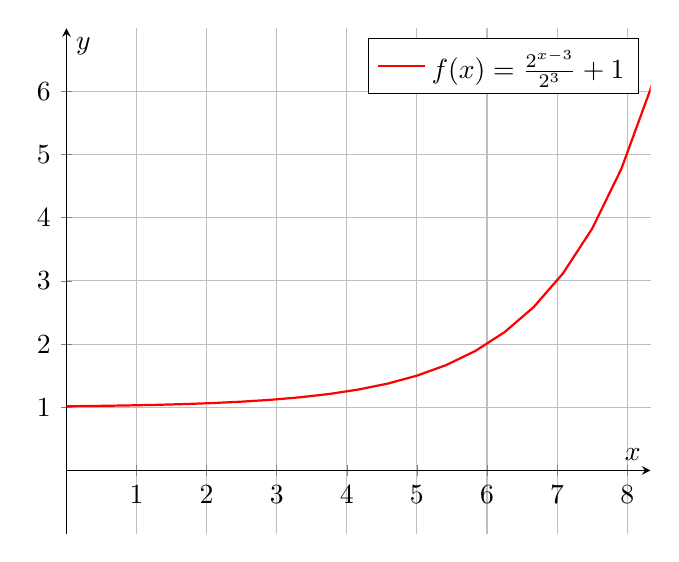
\begin{tikzpicture}
 		\begin{axis}[    %definiran koordinatni sistem, axis-mreža, parametri ločeni z vejicami
 			axis lines = middle,
 			domain = 0:10,
 			width = 9cm,
 			height = 8cm,
 			xtick = {0, 1, 2, 3, 4, 5, 6, 7, 8},
 			ytick = {0, 1, 2, 3, 4, 5, 6},
 			ymin = -1,
 			ymax = 7,
 			grid = both,
			xlabel = {$x$},
			ylabel = {$y$},
 		]
		\addplot[red, thick]{2^(x - 3)/2^3 + 1};
		\addlegendentry{$f(x)=\frac{2^{x - 3}}{2^3} + 1$}
 		\end{axis}
		
 	\end{tikzpicture}
 \end{frame}

\section{Paket \texttt{beamer} in tabele}
\begin{frame}{Odkrivanje tabele po vrsticah}
	Včasih pride prav, da tabelo odkrivamo postopoma po vrsticah.
	\begin{center}
		\begin{tabular}{c|cccc}
		   Oznaka & A & B & C & D \\ \hline \pause
		   X & 1 & 2 & 3 & 4 \\ \pause
		   Y & 3 & 4 & 5 & 6 \\ \pause
		   Z & 5 & 6 & 7 & 8
		\end{tabular}
	\end{center}
\end{frame}
 

\begin{frame}{Odkrivanje tabele po stolpcih}
	Tabelo lahko odkrivamo tudi po stolpcih, čeprav ni najlažje.

	\begin{center}
		\begin{tabular}{c|>{\onslide<2->}c>{\onslide<3->}c>{\onslide<4->}c>{\onslide<5->}c<{\onslide}}  %odkrivanje po stolpcih
		   Oznaka & A & B & C & D \\ \hline
		   X & 1 & 2 & 3 & 4 \\ 
		   Y & 3 & 4 & 5 & 6 \\
		   Z & 5 & 6 & 7 & 8
		\end{tabular}
	\end{center}
\end{frame}


\section[Matematika, 2. del\\\large{Zaporedja, algebra, grupe}]{Matematika, 2. del}
\begin{frame}{Zaporedja, vrste in limite}
	\begin{enumerate}
		\item 
		Naj bo $\sum_{n=1}^{\infty}$ $a_n$ absolutno konvergentna vrsta in $a_n \ne -1$.
		Dokaži, da je tudi vrsta $\sum_{n=1}^\infty \frac{a_n}{1+a_n}$
		absolutno konvergentna.

		\item
		Izračunaj limito
		$$ \lim_{x\to\infty } (\sin\sqrt{x+1} -\sin\sqrt{x}). $$

		\item
		Za dani zaporedji preveri, ali sta konvergentni.
		% Pomagajte si s spodnjima delno pripravljenima matematičnima izrazoma:
		$$
		 a_n = \underbrace{t\sqrt{2+\sqrt{2+\dots+\sqrt{2}}}}_{n korenov} \qquad
		 b_n = \underbrace{\sin(\sin(\dots(\sin 1)\dots))}_{n sinusov}
		$$
		
	\end{enumerate}
\end{frame}

\begin{frame}{Algebra}
	\begin{enumerate}
		\item
		Vektorja $\vec{c}= \vec{a} + \vec{2b}$ in $\vec{d}= \vec{a}-\vec{b}$
		sta pravokotna in imata dolžino 1. Določi kot med vektorjema $\vec{a}$ in $\vec{b}$.
		\item 
		Izračunaj $
		{\begin{pmatrix}
			1 & 2 & 3 & 4 & 5 & 6\\
            4 & 5 & 2 & 6 & 3 & 1
		\end{pmatrix}}^{-2000} $
		
	\end{enumerate}
\end{frame}

\begin{frame}{Velika determinanta}     %\cdots  \vdots  \ldots  \ddots
	Izračunaj naslednjo determinanto $2n \times 2n$, ki ima na neoznačenih mestih ničle.
	$$\begin{vmatrix}
		1 &  & & & 1& & & & \\
		&  2 & & & 2 & & & &    \\
		&  & \ddots & & \vdots & & & &     \\
		& &  & n-1 & n-1 & & & &     \\
		1 & 2 & \cdots & n-1& n & n+1& n+2& \cdots   & 2n      \\
		& & &  & n+1 & n+1 & & &     \\
		& &  & & n+2 & & n+2 & &     \\
		& & &  & \vdots& & & \ddots &     \\
		& &  & & 2n & & & & 2n     
    \end{vmatrix}$$
\end{frame}

\begin{frame}{Grupe}
	Naj bo 
	\begin{align*}
	G & = \{ z\in \mathbb{C};\; z = {2}^{k} (\cos(m\pi\sqrt{2})+ i \sin(m\pi\sqrt{2})), k, m \in \mathbb{Z}  \} \\
	H & = \{ (x,y) \in {\mathbb{R}}^{2}; x,y \in \mathbb{Z} \}
	\end{align*} 
	\begin{enumerate}
		\item
			Pokaži, da je $G$ podgrupa v grupi $ (\mathbb{C}\backslash \{0\}, \cdot)$
			neničelnih kompleksnih števil za običajno množenje.
		\item
			Pokaži, da je $H$ podgrupa v aditivni grupi $({\mathbb{R}}^{2}, +)$
			ravninskih vektorjev za običajno seštevanje po komponentah.
		\item
			Pokaži, da je preslikava $f:H\to G$, podana s pravilom
			$$
			(x,y) \mapsto {2}^{x}(\cos(y\pi\sqrt{2})+i\sin(y\pi\sqrt{2}))
			$$
			izomorfizem grup $G$ in $H$.
	\end{enumerate}
\end{frame}


\end{document}